\chapter{Vertikálna štruktúra aplikácie}

V~tejto kapitole uvádzame bližší pohľad na~súčasnú podobu hlavného okna a~session-ov aplikácie. Aktuálne aplikácia disponuje len jedným typom session-u určeným pre~samotné vyhľadávanie ciest v~mapách (\textit{Path finding session}). Viac informácií o~vertikálnej štruktúre aplikácie je možné nájsť v~Sekcii~\ref{sessions_hlavne_okno}.

\section{Hlavné okno}

O obecných úlohách hlavného okne sme sa zmienili už v~Podsekcii~\ref{Hlavne_okno_obecne}. V~tejto sekcii sa pozrieme na~aktuálne implementovanú architektúru, ako aj~funkcionalitu hlavného okna.


Hlavné okno je tvorené dvomi časťami: hlavným menu a~hlavnými nastaveniami.
Popri tom interaktívne využíva v~nastaveniach služby mechanizmu pre~správu výškových dát.

Ako už bolo spomenuté v~Podsekcii~\ref{Hlavne_okno_obecne}, po~zatvorení hlavného okna sa ukončuje aj~aplikácia. Tým pádom je úlohou hlavného okna zaistiť uloženie všetkých parametrov aplikácie pre~využitie v~budúcich behoch.

V~následujúcich podsekciách popíšeme časti, z~ktorých je aktuálne hlavné okno tvorené. Na~konci tejto sekcie je zobrazený Diagram~\ref{obr03:hlavne_okno} reprezentujúci jeho architektúru.

\subsection{Hlavné menu}

Hlavné menu je prvá časť, ktorá sa v~hlavnom okne užívateľovi po~zapnutí aplikácie zobrazí. Obsahuje možnosti vytvorenia inštancií session-ov a~možnosť otvorenia hlavných nastavení aplikácie. 

View model hlavného menu si vedie evidenciu všetkých otvorených session-ov. Pri~detekcii zatvorenia hlavného okna sa stará o~ich správne ukončenie. Taktiež si drží referenciu na~sprostredkovateľa hlavných nastavení. Toho následne môže predať session-om, ktorý~ho môžu použiť pre~získanie parametrov platných pre~celú aplikáciu.

Zvláštnosťou tejto časti je absencia vlastného model view-u. V~aktuálnej podobe aplikácie totiž nie je potrebný, nakoľko hlavné menu nepotrebuje komunikovať so~žiadnym modelom ani inou časťou hlavného okna. Ak by táto potreba v~budúcnosti vznikla, nemal by byť problém model view pre~hlavné menu vytvoriť. 

Možné vylepšenie tejto časti by mohlo zahrňovať vypísanie všetkých aktuálne otvorených session-ov pre~užívateľa. Zaistilo by to preňho jednoduchšiu orientáciu v~aplikácii.

\subsection{Hlavné nastavenia}

Hlavné nastavenia sú druhou časťou hlavného okna. Zabezpečujú možnosť pre~užívateľa nastaviť parametre, ktoré~sú využívané celou aplikáciou. 

V~aktuálnom stave sú to len dve možnosti konfigurácie: možnosť zmeny lokalizácie aplikácie a~možnosť nastavenia implicitne používaného zdroja výškových dát (presnejšie konkrétnej distribúcie výškových dát daného zdroja). 

Lokalizácia je implementovaná na~základe lokalizačných .resx zdrojových súborov. Avalonia je schopná takéto zdroje využívať aj~na~zmenu pevných nápisov aplikácie. %Ak nestihnem prelozit aplikaciu, tak to tu spomenut...ze z~casovych dovodov

Zdroj výškových dát je nastavovaný za~pomoci interakcie s~mechanizmom konfigurácie výškových dát. Po~stlačení príslušného tlačidla sa v~hlavnom okne zobrazí view zodpovedajúci tomuto mechanizmu. Užívateľ si v~ňom môže vybrať, ktorú distribúciu dát chce implicitne v~aplikácii využívať. Viac informácií ohľadom konfigurácie výškových dat nájdete v~následujúcej podsekcii.

Do budúcna sa počíta s~rozšírením hlavných nastavení do~takej miery, aby~sa z~nich dali konfigurovať aj~rôzne preferencie vo~vrstve Model. Pre~toto rozšírenie by sa však museli upraviť oblasti vrstvy Model, aby~tieto konfigurácie dokázali prijímať.

\subsection{Konfigurácia výškových dát}\label{konfiguracia_vyskovych_dat}

Konfigurácia výškových dát má špecifický spôsob využitia. Je určená na~to byť otváraná pomocou interakcie, vytvorenej inou časťou aplikácie. Jej hlavnou funkciou je dodávanie mechanizmu sťahovania a~mazania výškových dát, ktoré~je možné využiť ako dodatočný informačný zdroj pri~vytváraní mapových reprezentácií. 

Výškové dáta sú sťahované zo~špecifických zdrojov. Zdroje výškových dát môžu obsahovať viacero dátových distribúcií. Tie sa môžu líšiť v~kvalite, presnosti či~dostupnosti dodávaných výškových dát. 

Manipulácia s~dátami je vykonávaná po~oblastiach zvaných \textit{regióny}. Veľkosť a~tvar regiónov si každá distribúcia dát definuje sama. 

V~niektorých prípadoch zdroj výškových dát môže vyžadovať k~ich sprístupneniu autorizáciu užívateľa pomocou mena a~hesla. Táto autorizácia nemusí byť požadovaná pre~všetky jeho dátových distribúciach. V~prípade potreby autorizácie mechanizmus zabezpečuje možnosť užívateľovi dané údaje poskytnúť. Následne sa aplikácia pokúsi na~ich základe požadované dáta získať.   

Sťahovanie a~mazanie dát prebieha asynchrónne. Užívateľ je informovaný o~tom, ktoré~regióny su aktuálne stiahnuté, sťahované, neprítomné a~odstraňované. Viacero regiónov môže byť sťahovaných/odstraňovaných naraz, či~už z~jedného alebo~rôznych dátových zdrojov. Správne asynchrónne fungovanie manipulácie s~dátami zaručujú implementácie zdrojov výškových dát v~Model vrstve.

Špecifickou vlastnosťou konfigurácie výškových dát je možnosť ju používať súčasne z~viacerých miest v~aplikácii. Je navrhnutá tak, aby~zvládala korektne akceptovať pokyny z~mnohých interakcií naraz. Vďačí za~to návrhu model view-u, ktorý~poskytuje informácie o~tom, v~akom štádiu sťahovania sú jednotlivé regióny. Vďaka tomu všetky naviazané view model-y získajú aktuálne informácie a~môžu správne korigovať manipuláciu s~výškovými dátami.

Spôsob používania konfigurácie výškových dát je následovný:
\begin{itemize}
    \item Pri~inicializácii interakcie je novo vytvorenému view model-u(následne použitému v~interakcii) predaná aktuálne využívaná distribúcia výškových dát.
    \item Tá je v~konfigurácii nastavená ako aktuálne konfigurovaná a~ukázaná pomocou view-u užívateľovi.
    \item Následne prichádza fáza samotného konfigurovania výškových dát. Užívateľ môže:
    \begin{itemize}
        \item Zmeniť aktuálne konfigurovanú distribúciu výškových dát.
        \item Sťahovať a~odstraňovať výškové dáta aktuálne vybranej distribúcie. Tieto úkony sú uskutočňované na~základe regiónov, definovaných konfigurovanou distribúciou.
        \item Zadať autorizačné údaje pre~možnosť využitia dát zo~špecifických distribúcií, ktoré~autorizáciu vyžadujú. 
        \item Ukončiť konfiguračnú interakciu.
    \end{itemize} 
    \item Pri~ukončení interakcie sa posledne konfigurovaná distribúcia vráti ako novo zvolená na~používanie.
\end{itemize}

\begin{figure}[h]\centering
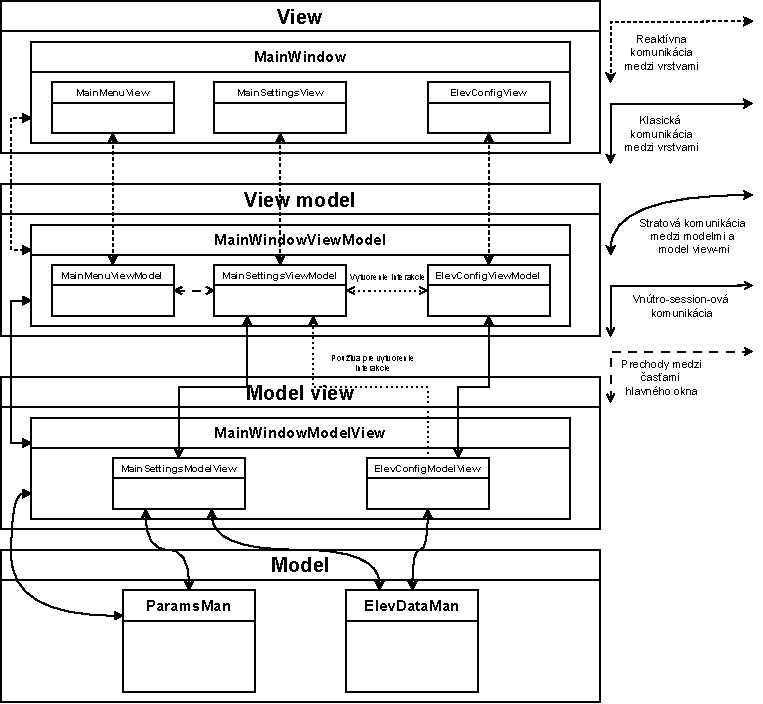
\includegraphics[]{img/hlavne_okno}
\caption{Diagram popisujúci architektúru hlavného okna aplikácie.} 
\label{obr03:hlavne_okno}
\end{figure}

\pagebreak

\section{Session pre~vyhľadávanie ciest v~mapách}

Vyhľadávanie ciest v~mapách je hlavnou náplňou aplikácie. V~tejto sekcii popíšeme typ session-u, ktorý~zabezpečuje logiku za~doručovaním tejto služby. Mechanizmus hľadania cesty v~mapách zahrnuje:
\begin{itemize}
    \item výber vstupných parametrov tak, aby~ich kombinácia bola platná, 
    \item vytvorenie grafickej reprezentácie mapy,
    \item vytvorenie mapovej reprezentácie, v~ktorej sa bude vyhľadávať cesta,   
    \item umožnenie užívateľovi zadať trať, na~ktorej sa má cesta vyhľadať,
    \item spustenie implementácie vybraného vyhľadávacieho algoritmu na~zvolenej trati a~vykreslenie nájdenej cesty. 
\end{itemize} 
V~aktuálnej podobe sa mechanizmus vyhľadávania cesty skladá z~troch častí: 
\begin{itemize}
    \item Nastavenie parametrov hľadania cesty (template, mapa, užívateľský model a~vyhľadávací algoritmus).
    \item Vytvorenie mapovej reprezentácie na~základe vybranej mapy a~template-u. Prípadne za~pomoci prítomných výškových dát. Táto časť je navrhnutá pre~použitie v~interakcii. Interakciu iniciuje časť nastavovania parametrov. 
    \item Spúšťanie zvoleného vyhľadávacieho algoritmu na~vytvorenej mapovej reprezentácii za~využitia výpočtov vybraného užívateľského modelu. Zahrňuje prijímanie trate od užívateľa a~vykreslovanie nájdenej cesty.
\end{itemize} 

Časť, ktorá sa z~časových dôvodov nedostala do~mechanizmu hľadania cesty je tzv. \textit{relevance-feedback} mechanizmus. Ten by slúžil pre~užívateľa na~dodatočné nastavenie hodnôt vybraného užívateľského modelu na~základe jeho preferencií vzhľadom k~aktuálne vybranej mape. Z~tejto časti zostal v~aplikácii len odpovedajúci model view, ktorý~v~tejto chvíli nenesie žiadnu užitočnú funkcionalitu. Slúži iba pre~prenos dát v~Model view vrstve. Bol v~aplikácii ponechaný z~dôvodu plánovaného budúceho rozšírenia aplikácie o~relevance-feedback mechanizmus.

V~následujúcich podsekciách popíšeme časti, z~ktorých je aktuálne session tvorený. Na~konci tejto sekcie je zobrazený Diagram~\ref{obr04:session_vyhladavania_cesty} reprezentujúci jeho architektúru.

\subsection{Nastavenia parametrov pre~vyhľadávanie cesty}

Nastavenia parametrov sú prvou časťou, ktorá je užívateľovi po~vytvorení session-u predostretá. Ten si za~jej pomoci zvolí:

\begin{itemize}
    \item template atribútov, ktoré~budú extrahované do~mapovej reprezentácie, 
    \item mapový súbor, na~základe ktorého sa bude vytvárať mapová reprezentácia. Teda súbor s~mapou, na~ktorej bude prebiehať vyhľadávanie ciest.
    \item súbor s~užívateľským modelom, ktorý~bude používaný algoritmom na~agregáciu hodnôt z~atribútov uložených v~mapovej reprezentácii  
    \item vyhľadávací algoritmus použitý na~hľadanie ciest v~mapovej reprezentácii za~pomoci výpočtov vybraného užívateľského modelu
\end{itemize}

Na začiatku sa predvolia parametre na~tie, ktoré~boli použité v~predchádzajúcej inštancii session-u. Uložené parametre prežívajú aj~samotné behy aplikácie.  

Vyberanie parametrov sa musí riadiť istými pravidlami z~dôvodu závislostí jednotlivých typov objektov, popísaných v~podsekciách Sekcie~\ref{Aspekty_hladania}. Danými pravidlami sú:
\begin{itemize}
    \item Jednotlivé parametre sa nastavujú postupne. Najprv je nutné, aby~bol vybraný mapový súbor a~template. Následne môže byť vybraný aj~súbor s~užívateľským modelom. Keď sú všetky tri predchádzajúce položky vybrané, je možné vybrať vyhľadávací algoritmus. 
    \item Pre~zvolenú kombináciu template-u a~formátu mapového súboru musí existovať mapová reprezentácia, ktorá túto kombináciu dokáže spracovať. Taktiež pre~zvolený template-u musí existovať typ užívateľského modelu, ktorý~dokáže spracovávať atribúty definované týmto template-om. Nakoniec musí existovať aspoň jedna kombinácia takto definovanej mapovej reprezentácie a~užívateľského modelu, ktorú dokáže využiť aspoň jedna implementácie ľubovoľného vyhľadávacieho algoritmu.   
    
    Keď je vybraný buďto template alebo~mapový súbor a~výber druhej položky by spôsobil neplatnú kombináciu, prvá položka sa opäť vynuluje. Možným vylepšením by bolo zabezpečenie indikácie platných kombinácií template-ov a~formátov mapových súborov.
    \item Súbor s~užívateľským modelom môže byť vybraný len takého typu, ktorý~dokáže spracovávať atribúty definované zvoleným template-om a~ktorý spolu s~ľubovoľnou mapovou reprezentáciou, ktorá dokáže spracovať aktuálne zvolenú kombináciu template-u a~mapového formátu, je použiteľnou kombináciou pre~aspoň jednu implementáciu nejakého vyhľadávacieho algoritmu. 
    \item Vyhľadávací algoritmus následne môže byť zvolený len taký, ktorý~dokáže využiť vybraný užívateľský model a~niektorú mapovú reprezentáciu, ktorú je možné vytvoriť z~vybraného template-u a~mapového súboru.
\end{itemize}    

Po výbere mapového súboru sa ihneď z~agregovanej mapy vytvorí jej grafická reprezentácia a~jej náhľad sa zobrazí užívateľovi.

Po dosadení všetkých parametrov môže užívateľ pokračovať do~ďalšej časti mechanizmu, ktorou je vytváranie mapovej reprezentácie. V~okamžiku prechodu do~tejto časti sa taktiež uložia aktuálne nastavené parametre, aby~mohli byť znovu použité ako predvolené v~následujúcich inštanciách session-u. 

Proces vytvárania mapovej reprezentácie je vykonaný za~pomoci interakcie z~parametre-nastavovacej časti. Na~základe jej výsledku sa následne buď presunieme v~mechanizme ďalej do~cestu-vyhľadávacej časti (úspešné vytvorenie) alebo~zostaneme v~nastaveniach.(neúspešné vytvorenie).  

\subsection{Vytváranie mapovej reprezentácie}

Vytváranie mapovej reprezentácie je akási prechodová časť medzi nastaveniami a~samotným vyhľadávaním ciest v~mape. Je prevedená za~pomoci interakcie iniciovanej v~nastaveniach, po~dosadení všetkých potrebných parametrov. Táto interakcia je spracovaná pomocou dialógového okna. Pomocou neho môže užívateľ pozorovať priebeh tvorby mapovej reprezentácie a~aktívne sa zapájať pri~riešení vzniknutých problémov.  

Priebeh tvorby mapovej reprezentácie je nasledovný:
\begin{itemize}
    \item Ihneď po~inicializácii tejto časti sa spustí proces kontroly podmienok tvorby mapovej reprezentácie. Aktuálne je využívaná iba kontrola prítomnosti potrebných výškových dát pri~procese tvorenia mapovej reprezentácie. (Táto kontrola zahrňuje aj~schopnosť mapy dodať informácie o~svojej pozícii a~rozlohe, ktoré~sú nevyhnutné pre~získanie odpovedajúcich výškových dát).
    
    Pokiaľ tvorená mapová reprezentácia indikuje potrebu výškových dát, skontroluje sa, či~sú odpovedajúce dáta prítomné. Pokiaľ dáta prítomné niesu alebo~mapa nie je schopná definovať svoju geografickú polohu/rozlohu, vytváranie mapovej reprezentácie zlyhá a~užívateľ sa môže vrátiť do~nastavení. 
    
    Do~budúcna je v~pláne umožniť užívateľovi riešenie problému nedostatku výškových dát za~pomoci interakcie s~konfiguráciou výškových dát. Viac informácii o~konfigurácii výškových dát je možné nájsť v~Podsekcii~\ref{konfiguracia_vyskovych_dat}.
    \item Pokiaľ kontrola podmienok dobehne úspešne, je automaticky spustený proces vytvárania mapovej reprezentácie. Tento proces môže trvať dlhšiu dobu a~teda je užívateľovi umožnené sledovať jeho vývoj alebo~ho dokonca prerušiť. Po~prerušení je užívateľ vrátený naspäť do~nastavení parametrov.
\end{itemize}

\subsection{Vyhľadávanie cesty v~mape}

Po úspešnom vytvorení mapovej reprezentácie sa môžeme presunúť k~samotnému vyhľadávaniu ciest v~mape. V~tejto chvíli máme k~dispozícii všetky potrebné dátové zdroje k~správnemu vykonávaniu tejto činnosti.

Na začiatku je vykreslená grafika mapy, ktorá bola vytvorená v~nastaveniach pri~výbere mapového súboru.

Kolobeh vyhľadávania je rozdelený do~troch fáz:
\begin{itemize}
    \item Prvou fázou je umožnenie výberu trate užívateľovi. Trať sa skladá z~postupností bodov, medzi ktorými je následne vyhľadávaná cesta. Užívateľ môže pridávať a~odoberať koncové body trate.
    \item Po~zadaní cesty prichádza na~rad fáza samotného vyhľadávanie cesty. Algoritmus má možnosť podávať správy o~postupe vyhľadávania, či~už pomocou textovej informácie alebo~grafického znázorňovania. Užívateľ mám možnosť proces vyhľadávania predčasne ukončiť. V~takom prípade sa kolobeh vráti do~prvej fázy výberu trate.
    \item Pokiaľ vyhľadávania cesty dobehne úspešne, príde na~rad tretia fáza, ktorou je vykreslenie nájdenej cesty. Zároveň sa po~strane môžu vypísať informácie o~nájdenej trase (napríklad jej dĺžka, prekonané prevýšenie, atď.). V~tejto fáze je užívateľovi umožnené interagovať s~nájdenými cestami (s takými, ktoré~takúto funkcionalitu zabezpečujú). Po~dokončení prezerania nájdenej cesty sa opäť vrátime do~prvej fázy výberu trate.  
\end{itemize}

Počas ktorejkoľvek fázy je užívateľ schopný približovať, odďalovať a~hýbať so~zobrazenou grafikou vyhľadávania.

\begin{figure}[h]\centering
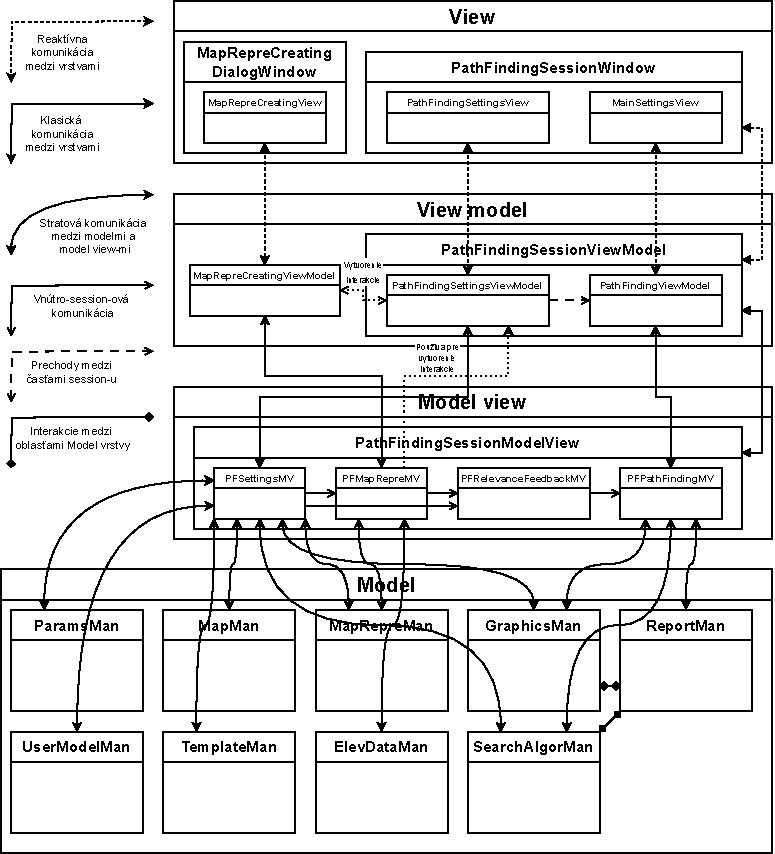
\includegraphics[]{img/session_vyhladavania_cesty}
\caption{Diagram popisujúci architektúru session-u pre~vyhľadávanie cesty v~mapách} 
\label{obr04:session_vyhladavania_cesty}
\end{figure}

% \subsection{Zaujímavé implementačné postupy} % % V~tejto podsekcii vymenujeme pár zaujímavých postupov využitých pri~implementácii \textit{hlavného okna}.  % \begin{itemize} % \item \textbf{Zatváranie hlavného okna} - zatváranie hlavného okna je špecifické tým, že~ukončuje beh celej aplikácie. Preto je v~niektorých prípadoch potrebné, aby~bolo možné sa opýtať užívateľa, či~si je istý svojou požiadavkou na~ukončenie aplikácie. Ideálnym spôsobom na~zistenie užívateľovho názoru je použitie dialógového okna. Ač sa to môže zdať ako triviálna úloha, s~Avalonia framework-om to zas tak jednoduché nebolo.  % % Následujúci kód ukazuje nefunkčný príklad \texttt{MainWindow\_OnClosing} metódy z~triedy \texttt{MainWindow} určenej na~zachytávanie a~spracovanie udalosti zatvárania hlavného okna: % % \begin{lstlisting} % private async void MainWindow_OnClosing % (object? sender, WindowClosingEventArgs e) % { % bool close = % await ViewModel!.OnClosingCommand.Execute(); % if (!close) % { % e.Cancel = true; % } % } % \end{lstlisting} % 
    % Na~prvý pohľad by sa mohlo zdať že~je všetko v~poriadku. Pokiaľ spustený \texttt{ViewModel.OnClosingCommand} vráti indikáciu toho, že~sa okno nesmie zavrieť, nastaví sa vlastnosť \texttt{Cancel} na~true a~tým sa zabráni zatvoreniu hlavného okna.
    % 
    % Problém je však v~tom, že~spustenie daného príkazu na~view modelu prebieha asynchrónne z~dôvodu možnosti otvorenia dialógového okna na~komunikáciu s~užívateľom. Výsledok príkazu je potrebné očakávať za~pomoci kľúčového slova \texttt{await}, nakoľko jeho použitie zabezpečí, že~UI thread zostane aktívne a~reagujúce.
    % 
    % To však na~druhú stranu sa stáva problémom, nakoľko UI spracuje argument \texttt{e} prv než naša metóda dokáže správne dosadiť jeho vlastnosť \texttt{Cancel}. Teda okno sa zavrie skorej, než je užívateľovi daná možnosť to zvrátiť.
    % 
    % Preto bol použitý následujúci návrh metódy, ktorý~zaručuje správny spôsob zatvárania hlavného okna:
    % \begin{lstlisting}
    % private bool _alreadyAsked = false;
    % private async void MainWindow_OnClosing
        % (object? sender, WindowClosingEventArgs e)
    % {
        % if (_alreadyAsked) return;
        % e.Cancel = true;
        % bool close = 
            % await ViewModel!.OnClosingCommand.Execute();
        % if (close)
        % {
            % _alreadyAsked = true;
            % Close();
        % }
    % }
    % \end{lstlisting}
% 
    % v~tomto prípade sme predošlý problém vyriešili malým trikom. Vždy keď zaznamenáme udalosť zatvárania okna iniciovanú užívateľom, nastavíme automaticky príznak \texttt{Cancel} argumentu \texttt{e} na~true. Tým zabránime predčasnému zatvoreniu okna. 
    % 
    % Následne podobne ako v~predošlom prípade asynchronne zavoláme spustenie \texttt{ViewModle.OnClosingCommand} a~počkáme na~výsledný indikátor. Ak indikuje pokračovanie v~zatváraní aplikácie, príde na~radu náš trik.  
% 
    % Nastavíme hodnotu, k~tomuto špecifickému účelu vytvoreného, privátneho poľa \texttt{\_alreadyAsked} na~true. Toto pole indikuje, že~sa hlavné okno už raz užívateľa pýtalo na~jeho názor na~zatvorenie aplikácie a~že jeho odpoveď bola pozitívna. 
    % 
    % Po~nastavení poľa je opäť zavolaná metóda Close() na~hlavnom okne. Na~základe tohto volania sa opäť hlavné okno pokúsi zavrieť. Tým pádom sa znova zavolá metóda \texttt{MainWindow\_OnClosing}. Tentokrát sa však jej beh zastaví hneď na~začiatku na~dotaze, či~pole \texttt{\_alreadyAsked} indikuje už zistený užívateľov súhlas so~zavretím okna. Tým pádom sa vlastnosť \texttt{Cancel} nestihne nastaviť na~true a~teda hlavné okno sa následne zavrie.    
% 
    % Tento princíp je možné využiť taktiež v~ostatných oknách aplikácie, ak by mali potrebu rovnakého mechanizmu ich zatvárania. 
    % \item \textbf{Súbežné využívanie inštancie \texttt{ElevDataModelView}-u} - za~možnosťou súbežného využívania model view-u konfigurácie výškových dát je malý trik. Na~začiatok je potrebné si uvedomiť, ktoré~dáta je potrebné držať synchrónne vo~všetkých používaných konfiguráciách výškových dát a~ktoré na~druhú stranu majú byť pre~každú konfiguráciu jedinečné:
    % \begin{itemize}
        % \item Synchrónne je potrebné držať informácie o~stave prítomnosti jednotlivých regiónov všetkých distribúcií. Keby sa v~týchto dátach objavila akákoľvek nesúmernosť, mohlo by to mať fatálne dôsledky na~manipuláciu s~výškovými dátami.
        % \item Na~druhú stranu každá konfigurácia by si mala sama určovať, ktorá distribúcia výškových dát je aktuálne konfigurovaná. Predsa len to je jedným zo~zámerov procesu konfigurácie. Nechať užívateľa vybrať ním žiadanú distribúciu na~použitie či~upravenie.
    % \end{itemize}
% 
    % Teda potrebujeme, aby~inštancia \texttt{ElevDataModelView} v~sebe držala informáciu o~prítomnosti jednotlivých regiónov pre~všetky distribúcie. Pre~konkrétny región je táto informácia uložená v~data view modele, do~ktorého je príslušný región zabalený (viac informácií k~data view modelom nájdete v~podsekcii~\ref{ViewModel}). Samotný región si nesie informáciu len o~tom, či~sú preňho dáta stiahnuté alebo~nie. Neinformuje ale~o~tom, čí sú dáta aktuálne sťahované alebo~odstraňované.
% 
    % Typicky model view-y vytvárajú vždy nový data view model pre~každý údaj získaný z~Model vrstvy v~momente posúvanie jeho informácie do~vrstvy View model. Tu však prichádza na~rad malý trik, kedy \texttt{ElevDataModelView} vytvorí data view modely pre~všetky existujúce regióny počas svojej inicializácie a~uloží ich do~slovníka \texttt{TopRegionsOfAllDistributions}. Následne je tento slovník ponúkaný všetkým inštanciám triedy \texttt{ElevConfigViewModel} a~teda všetky tieto inštancie pracujú s~jednými a~tými istými objektmi regiónových data view modelov.
    % 
    % Tým pádom všetky inštancie triedy \texttt{ElevConfigViewModel} zdieľajú informácie o~stave prítomnosti jednotlivých regiónov a~teda nemôže nastať nekonzistencia v~akciách manipulujúcich s~výškovými dátami. (samozrejme za~predpokladu, že~užívateľ nie je schopný stlačiť dve tlačidlá v~rôznych konfiguračných oknách v~ten istý moment. Pri~klasickom používaní aplikácie by tento scenár nikdy nemal nastať).
% 
    % Na~druhú stranu každá inštancia triedy \texttt{ElevConfigViewModel} si sama drží informáciu o~aktuálne konfigurovanej distribúcii výškových dát a~teda v~každej z~týchto inštancií môžem v~rovnakom čase konfigurovať inú distribúciu.
% \end{itemize}










% \subsection{Zaujímavé implementačné postupy}
% 
% v~tejto podsekcii vymenujeme pár zaujímavých postupov využitých pri~implementácii \textit{session-u pre~vyhľadávanie ciest v~mapách}.  
% 
% \begin{itemize}
    % \item \textbf{Spôsob zabezpečenia vnútornej komunikácie model view-ov} - Jednou z~náplní Model view vrstvy je zabezpečovať vnútro-session-ovú komunikáciu. Nikto okrem samotných model view-ov by nemal mať k~tejto komunikácii prístup. Okolie by mal mať možnosť vidieť iba metódy, ktorými Model view vrstva sprístupňuje svoje služby. 
    % 
    % Následujúca implementácia zaručuje ukrytie vnútornej komunikácie model view-ov cesty-vyhľadávacieho session-u. Môže slúžiť ako príklad pre~implementáciu Model view vrstvy ostatných session-ov. 
% 
    % Model view inštancie pre~daný session inicializuje \textit{session model view}. Ten ich následne aj~distribuuje do~ostatných potrebných častí session-u. 
    % 
    % Chyták však je, že~vytvárané inštancie niesu typu, ktorý~je navonok prezentovaný. Session model view definuje privátnych potomkov týchto prezentovaných typov, ktorí majú, narozdiel od ich predkov, implementovanú funkcionalitu vzájomnej komunikácie. Taktiež override-ujú všetku funkcionalitu predkov, v~ktorej je potrebná práca s~dátami prúdiacimi vo~vnútornej komunikácii.
% 
    % Tým že~sú tieto \uv{intra} triedy definované ako privátne, nie je možné mimo name-space-u session model view-u sledovať ich komunikáciu.
% 
    % \begin{listing}[h]
    % \begin{lstlisting}
    % public class PathFindingSessionModelView : SessionModelView
    % {
        % public PFSettingsMV Settings { get; }
        % public PFMapRepreCreatingMV MapRepreCreating { get; }
        % public PFRelevanceFeedbackMV RelevanceFeedback { get; }
        % public PFPathFindingMV PathFinding { get; }
        % 
        % public PathFindingSessionModelView()
        % {
            % var setI = new PFSettingsIntraMV();
            % var graCreI = new PFMapRepCreIntraMV(setI);
            % var relFeeI = 
                % new PFRelevanceFeedbackIntraMV(setI, graCreI);
            % var patFinI = new PFPathFindingIntraMV(relFeeI);
% 
            % Settings = setI;
            % MapRepreCreating = graCreI;
            % RelevanceFeedback = relFeeI;
            % PathFinding = patFinI;
        % }
        % private class PFSettingsIntraMV : PFSettingsMV        
        % private class PFMapRepreCreatingIntraMV : 
            % PFMapRepreCreatingMV
        % private class PFRelevanceFeedbackIntraMV : 
            % PFRelevanceFeedbackMV
        % private class PFPathFindingIntraMV : PFPathFindingMV
    % }
% 
    % public abstract class PFSettingsMV : ModelViewBase { }        
    % public abstract class PFMapRepreCreatingMV : 
        % ModelViewBase { }        
    % public abstract class PFRelevanceFeedbackMV : 
        % ModelViewBase { }
    % public abstract class PFPathFindingMV : ModelViewBase { }      
    % \end{lstlisting}
    % \caption{Príklad návrhu session model view-u, ktorý~skrýva vnútornú komunikáciu (upravený \texttt{PathFindingSessionModelView})}
    % \end{listing}
% 
% \end{itemize}